%%%%%%%%%%%%%%%%%%%%%%%%%%%%%%%%%%%%%%%%%
% Journal Article
% LaTeX Template
% Version 2.0 (February 7, 2023)
%
% This template originates from:
% https://www.LaTeXTemplates.com
%
% Author:
% Vel (vel@latextemplates.com)
%
% License:
% CC BY-NC-SA 4.0 (https://creativecommons.org/licenses/by-nc-sa/4.0/)
%
% NOTE: The bibliography needs to be compiled using the biber engine.
%
%%%%%%%%%%%%%%%%%%%%%%%%%%%%%%%%%%%%%%%%%

%----------------------------------------------------------------------------------------
%	PACKAGES AND OTHER DOCUMENT CONFIGURATIONS
%----------------------------------------------------------------------------------------

\documentclass[
	a4paper, % Paper size, use either a4paper or letterpaper
	10pt, % Default font size, can also use 11pt or 12pt, although this is not recommended
	unnumberedsections, % Comment to enable section numbering
	twoside, % Two side traditional mode where headers and footers change between odd and even pages, comment this option to make them fixed
]{LTJournalArticle}

\addbibresource{sample.bib} % BibLaTeX bibliography file

\runninghead{Deciphering Public Opinion} % A shortened article title to appear in the running head, leave this command empty for no running head


\setcounter{page}{1} % The page number of the first page, set this to a higher number if the article is to be part of an issue or larger work

%----------------------------------------------------------------------------------------
%	TITLE SECTION
%----------------------------------------------------------------------------------------

\title{Deciphering Public Opinion: A CRISP-DM Analysis of Reviews on Instagram's Threads App} % Article title, use manual lines breaks (\\) to beautify the layout

% Authors are listed in a comma-separated list with superscript numbers indicating affiliations
% \thanks{} is used for any text that should be placed in a footnote on the first page, such as the corresponding author's email, journal acceptance dates, a copyright/license notice, keywords, etc
\author{%
	Kelly Nguyen\thanks{Corresponding author: \href{mailto:kelly.nguyen01@sjsu.edu}{kelly.nguyen01@sjsu.edu}\\ \textbf{Received:} September 21, 2023, \textbf{Published:} September 21, 2023}
}

% Affiliations are output in the \date{} command
\date{\footnotesize\textsuperscript{\textbf{1}}Charles Davidson School of Engineering, \\San Jose State University, San Jose, California}

% Full-width abstract
\renewcommand{\maketitlehookd}{%
	\begin{abstract}
		\noindent As social media platforms evolve, understanding user sentiment becomes pivotal for enhancing user experience and driving engagement. Instagram's Threads app, designed for more intimate sharing among close friends, is the subject of this study. Utilizing the Cross-Industry Standard Process for Data Mining (CRISP-DM), we explored public opinion by analyzing a dataset of user reviews. The study involves data preparation, text mining, sentiment analysis, and predictive modeling. Our findings reveal key trends in user sentiment and specific features of the app that contribute to user satisfaction and dissatisfaction. The results offer actionable insights that could inform app developers, marketers, and policy-makers in their decision-making processes.
	\end{abstract}
}

%----------------------------------------------------------------------------------------

\begin{document}

\maketitle % Output the title section

%----------------------------------------------------------------------------------------
%	ARTICLE CONTENTS
%----------------------------------------------------------------------------------------

\section{Introduction}

Social media platforms have revolutionized the way we communicate, share information, and even perceive the world around us. The advent of specialized social networking apps has led to more nuanced ways of interaction, tailored to specific communication needs. Instagram, a leader in the visual social networking space, recently launched Threads, a new app aimed at fostering closer connections among friends. Despite the buzz surrounding its release, the question remains: What do users genuinely think about Threads?

Understanding public opinion about a social media app like Threads is not just an academic exercise; it has substantial implications for user experience, marketing strategies, and even the platform's long-term sustainability. Yet, capturing and deciphering such opinions from a sea of user reviews is a complex endeavor. The challenge lies in the multidimensionality of human sentiments and the vast volume of data.

To dissect this complexity, we employed the Cross-Industry Standard Process for Data Mining (CRISP-DM), a structured data analysis methodology that is widely respected for its effectiveness in converting raw data into valuable insights. This paper aims to explore the following research questions:
\begin{enumerate}
	\item What are the general sentiments expressed in user reviews of Instagram's Threads app?
	\item Are there specific features of the app that contribute to user satisfaction or dissatisfaction?
	\item Can we build predictive models that effectively gauge public sentiment based on user reviews?
\end{enumerate}
By the end of this paper, we aim to provide actionable insights gleaned from user reviews of Instagram's Threads app, offering a valuable resource for a diverse audience including app developers, digital marketers, and researchers in the fields of data science and social media analytics.

\section{CRISP-DM Methodology}

The Cross-Industry Standard Process for Data Mining (CRISP-DM) serves as the backbone of our research approach. This well-established methodology provides a structured framework for planning, implementing, and deploying data mining projects. It consists of five interconnected phases, each contributing to the overall goal of transforming raw data into actionable knowledge. These stages are:
\begin{enumerate}
	\item Business Understanding
	\item Data Acquisition and Understanding
	\item Data Preparation
        \item Hypothesis and Modeling
        \item Deployment, Operations and Maintenance
\end{enumerate}
\subsection{1. Business Understanding}
Business Understanding outlines the general business understanding and role of the data. This sector requires actionable information. The following sections outline the stages of the process. First is determining business  
objectives using the SMART approach which stands for specific, measurable, attainable, relevant, and timely. This often is performed by business stakeholders. This is typically a business success criteria, or a benchmark of threshold values. Then the situation is assessed, looking at the inventory of resources, requirements, assumptions and constraints. Risks, Contingencies, Costs, and Benefits are also assessed. Next is determining the goals of data mining and then producing a project plan.

\subsection{2. Data Acquisition and Understanding}
In this phase, data collection occurred based on the project requirements. Exploratory Data Analysis (EDA) was performed to understand the structure, patterns, and anomalies in the data. Typically the stages in this process include collection initial data, describing the data, exploring it, and the verifying the quality.

\subsection{3. Data Preparation}
During data preparation, data was cleansed, transformed, and formatted to be suitable for modeling. This phase often involves handling missing data, outliers, and feature engineering.
\subsection{4. Hypothesis and Modeling}
After preparing the data, we applied statistical, machine learning, or data mining techniques to the prepared data to create models that could predict or explain the problem we were interested in. Multiple models may be developed and compared.
\subsection{5. Deployment, Operations and Maintenance}
The final models are integrated into the operational systems, dashboards, or decision-making processes. Alternatively, the findings might be reported for strategic planning or other business purposes.

\subsection{Data Analysis}

Based on the initial data set examination, here are some key observations:The data set contains 40,435 entries, there are four columns: source, review description, rating, and review date, and all columns are non-null, indicating there are no missing values in the data set. The data types that exist are source and review description, which are object types and rating which is an integer. Review date is an object type but should ideally be a date time object for easier manipulation.
\begin{figure}
    \centering
    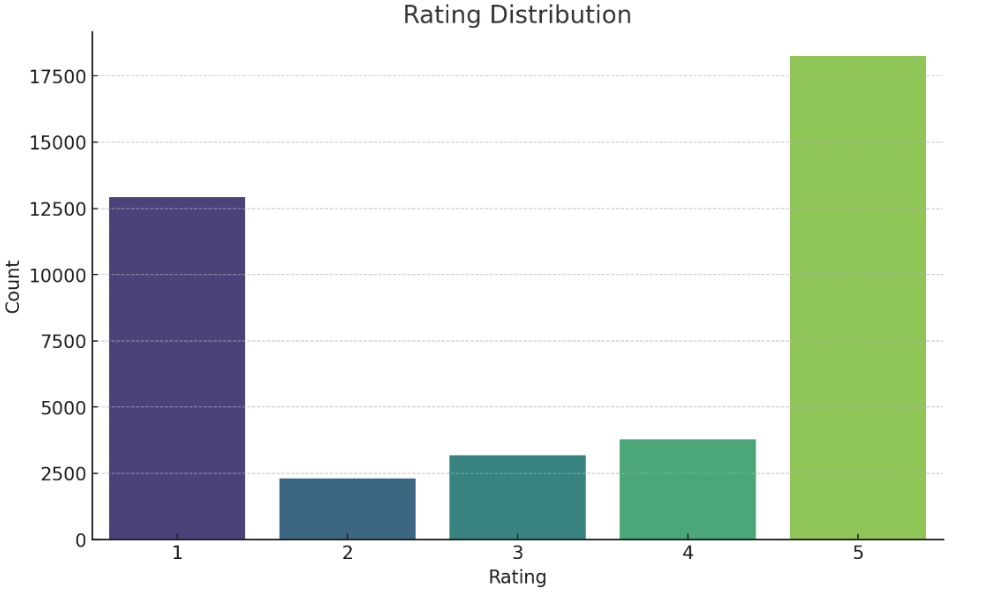
\includegraphics[width=1\linewidth]{Figures/Rating_distribution.png}
    \caption{Distribution of ratings}
    \label{fig:1}
\end{figure}


Referencing Figure \ref{fig:1}.
Furthering the data understanding, a plot was created which has the rating column ranges from 1 to 5 and the mean rating is approximately 3.3, with a standard deviation of 1.77. The 25th percentile (Q1) is 1, the median (Q2) is 4, and the 75th percentile (Q3) is 5. Furthermore the dataset contains reviews from two sources: Google Play (36,687 entries) and App Store (3,748 entries). We also were able to establish that ratings are skewed towards 5 (18,253 entries) and 1 (12,921 entries), indicating extreme opinions are more common. Initially as the data was viewed, the rating distribution plot confirms that ratings are mostly polarized towards 1 and 5.
As we prepared the data there were a few things that were noticed. As we checked for inconsistencies, there are no unusual ratings (all ratings are between 1 and 5) and no future dates in the review date column, which is a good sign of data integrity. Referencing Figure \ref{fig:2}.The box plot for ratings doesn't show any outliers, which is consistent with the nature of the rating system (1 to 5).
\begin{figure}
    \centering
    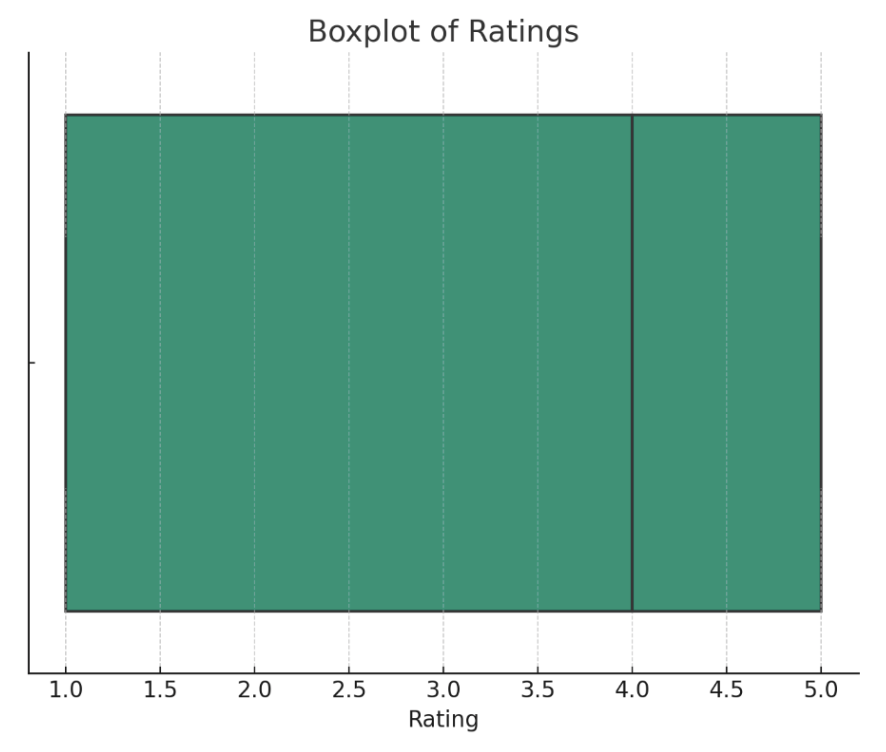
\includegraphics[width=1\linewidth]{Figures/boxplot.png}
    \caption{Outlier Box Plot}
    \label{fig:2}
\end{figure}


For modeling and evaluation, three different types of regression models to predict reviews: Linear Regression, Ridge Regression, and Lasso Regression. The metrics used to evaluate each model include Mean Squared Error (MSE), Mean Absolute Error (MAE) and R2 Score.
Referencing Table 1.

\begin{table*} % Full width table (notice the starred environment)
	\caption{Regression Model Results}
	\centering % Horizontally center the table
	\begin{tabular}{L{0.10\linewidth} R{0.2\linewidth} R{0.2\linewidth} R{0.2\linewidth}} % Manually specify column alignments with L{}, R{} or C{} and widths as a fixed amount, usually as a proportion of \linewidth
		\toprule
		Metric & Linear Regression & Ridge Regression & Lasso Regression \\
		\midrule
		MSE & 3.018 & 3.018 & 3.031\\
         MAE & 1.608 & 1.608 & 1.616 \\
         R2 Score & 0.038 & 0.038 & 0.034\\
		\bottomrule
	\end{tabular}
\end{table*}
%------------------------------------------------

\section{Summary and Findings}

Based on the CRISP-DM method that was just evaluated on the dataset, we found these conclusions. The dataset contained reviews from Google Play and the App Store, with the majority of ratings being either 1 or 5. We went through a detailed data preparation process that involved text preprocessing, feature engineering, and clustering. And lastly, three regression models were built to predict the review ratings. However, none of these models were highly effective, as indicated by the evaluation metrics. The current feature set is simplistic. More sophisticated features, possibly derived from the review text using techniques like TF-IDF or sentiment analysis, could improve model performance.

Based on the initial exploratory data analysis, the sentiment regarding the Threads app appears to be highly polarized. A significant number of reviews have either a 1-star or a 5-star rating, with fewer reviews in the 2, 3, or 4-star categories. This suggests that users either love the app or have significant issues with it. However, without detailed text analytics on the review description, it's challenging to pinpoint the exact sentiments.

The data set we have doesn't provide detailed information about specific features of the app that contribute to user satisfaction or dissatisfaction. While we did some text pre-processing on the review description, more advanced techniques like sentiment analysis, topic modeling, or keyword extraction would be needed to identify specific features that users mention positively or negatively.

Based on the models we built and the features we used, the predictive power was modest, with R2 scores around 0.038. This suggests that the models are not very effective at predicting user ratings based on the features engineered. However, this could be due to the simplicity of the features used. More advanced feature engineering, especially from the review text, could potentially lead to more effective models for gauging public sentiment.

To summarize, while the dataset provides some initial insights into user sentiment, more advanced techniques are needed to deeply understand specific aspects of user satisfaction or dissatisfaction and to build effective predictive models.

%------------------------------------------------

\section{Future Work}

For future analysis of the dataset, on top of the CRISP-DM process, a sentiment analysis which  incorporates sentiment as a feature, could add significant predictive power to the models. A temporal analysis could also have been done, which takes a look at time-based patterns that may have existed in the reviews. Lastly, taking a more in depth look at user behavior.If user-specific data is available, understanding user behavior could provide more personalized insights.

%----------------------------------------------------------------------------------------
%	 REFERENCES
%----------------------------------------------------------------------------------------

\begin{thebibliography}{9}

\bibitem{crispdm}
CRISP-DM 1.0,
\emph{CRISP-DM: Step-by-step data mining guide},
SPSS Inc.,
2000.

\bibitem{pandas}
Wes McKinney,
\emph{pandas: a foundational Python library for data analysis and statistics},
Python for Data Analysis,
O'Reilly Media,
2012.

\bibitem{sklearn}
F. Pedregosa, G. Varoquaux, A. Gramfort, et al.,
\emph{Scikit-learn: Machine Learning in Python},
Journal of Machine Learning Research,
2011.

\bibitem{nltk}
Steven Bird, Ewan Klein, and Edward Loper,
\emph{Natural Language Processing with Python},
O'Reilly Media,
2009.

\bibitem{matplotlib}
John D. Hunter,
\emph{Matplotlib: A 2D Graphics Environment},
Computing in Science \& Engineering,
2007.

\bibitem{seaborn}
Michael Waskom et al.,
\emph{seaborn: statistical data visualization},
Journal of Open Source Software,
2021.

\bibitem{regressionanalysis}
D. G. Kleinbaum and M. Klein,
\emph{Applied Regression Analysis and Other Multivariable Methods},
Cengage Learning,
2014.

\bibitem{featureselection}
I. Guyon and A. Elisseeff,
\emph{An Introduction to Variable and Feature Selection},
Journal of Machine Learning Research,
2003.

\bibitem{textmining}
Feldman, R. and Sanger, J.,
\emph{The Text Mining Handbook: Advanced Approaches in Analyzing Unstructured Data},
Cambridge University Press,
2007.

\end{thebibliography}


%----------------------------------------------------------------------------------------

\end{document}
